% Options for packages loaded elsewhere
\PassOptionsToPackage{unicode}{hyperref}
\PassOptionsToPackage{hyphens}{url}
%
\documentclass[
]{article}
\usepackage{amsmath,amssymb}
\usepackage{lmodern}
\usepackage{iftex}
\ifPDFTeX
  \usepackage[T1]{fontenc}
  \usepackage[utf8]{inputenc}
  \usepackage{textcomp} % provide euro and other symbols
\else % if luatex or xetex
  \usepackage{unicode-math}
  \defaultfontfeatures{Scale=MatchLowercase}
  \defaultfontfeatures[\rmfamily]{Ligatures=TeX,Scale=1}
\fi
% Use upquote if available, for straight quotes in verbatim environments
\IfFileExists{upquote.sty}{\usepackage{upquote}}{}
\IfFileExists{microtype.sty}{% use microtype if available
  \usepackage[]{microtype}
  \UseMicrotypeSet[protrusion]{basicmath} % disable protrusion for tt fonts
}{}
\makeatletter
\@ifundefined{KOMAClassName}{% if non-KOMA class
  \IfFileExists{parskip.sty}{%
    \usepackage{parskip}
  }{% else
    \setlength{\parindent}{0pt}
    \setlength{\parskip}{6pt plus 2pt minus 1pt}}
}{% if KOMA class
  \KOMAoptions{parskip=half}}
\makeatother
\usepackage{xcolor}
\usepackage[margin=1in]{geometry}
\usepackage{longtable,booktabs,array}
\usepackage{calc} % for calculating minipage widths
% Correct order of tables after \paragraph or \subparagraph
\usepackage{etoolbox}
\makeatletter
\patchcmd\longtable{\par}{\if@noskipsec\mbox{}\fi\par}{}{}
\makeatother
% Allow footnotes in longtable head/foot
\IfFileExists{footnotehyper.sty}{\usepackage{footnotehyper}}{\usepackage{footnote}}
\makesavenoteenv{longtable}
\usepackage{graphicx}
\makeatletter
\def\maxwidth{\ifdim\Gin@nat@width>\linewidth\linewidth\else\Gin@nat@width\fi}
\def\maxheight{\ifdim\Gin@nat@height>\textheight\textheight\else\Gin@nat@height\fi}
\makeatother
% Scale images if necessary, so that they will not overflow the page
% margins by default, and it is still possible to overwrite the defaults
% using explicit options in \includegraphics[width, height, ...]{}
\setkeys{Gin}{width=\maxwidth,height=\maxheight,keepaspectratio}
% Set default figure placement to htbp
\makeatletter
\def\fps@figure{htbp}
\makeatother
\setlength{\emergencystretch}{3em} % prevent overfull lines
\providecommand{\tightlist}{%
  \setlength{\itemsep}{0pt}\setlength{\parskip}{0pt}}
\setcounter{secnumdepth}{5}
\usepackage{amsmath}
\usepackage{hyperref}
\hypersetup{colorlinks = true, linkcolor = red, urlcolor = blue}
\usepackage{mathtools}
\usepackage{graphicx}
\PassOptionsToPackage{hyphens}{url}\usepackage{hyperref}
\usepackage[singlelinecheck=false]{caption}
\usepackage{booktabs}
\usepackage{longtable}
\usepackage{array}
\usepackage{multirow}
\usepackage{wrapfig}
\usepackage{float}
\usepackage{colortbl}
\usepackage{pdflscape}
\usepackage{tabu}
\usepackage{threeparttable}
\usepackage{threeparttablex}
\usepackage[normalem]{ulem}
\usepackage{makecell}
\usepackage{xcolor}
\ifLuaTeX
  \usepackage{selnolig}  % disable illegal ligatures
\fi
\IfFileExists{bookmark.sty}{\usepackage{bookmark}}{\usepackage{hyperref}}
\IfFileExists{xurl.sty}{\usepackage{xurl}}{} % add URL line breaks if available
\urlstyle{same} % disable monospaced font for URLs
\hypersetup{
  pdftitle={Supplementary Materials; Study on User-Controlled Radial Tour},
  pdfauthor={Nicholas Spyrison, Dianne Cook, Kim Marriott},
  hidelinks,
  pdfcreator={LaTeX via pandoc}}

\title{Supplementary Materials; Study on User-Controlled Radial Tour}
\author{Nicholas Spyrison, Dianne Cook, Kim Marriott}
\date{}

\begin{document}
\maketitle

This section covers some auxiliary details for the data simulation and collection. It continues on with an illustration of the visual methods and the demographics of the participants. Lastly, a parallel modeling analysis on log response time is conducted.

\hypertarget{data-simulation}{%
\subsection{Data simulation}\label{data-simulation}}

Each dimension is distributed initially as \(\mathcal{N}(0, 1)\), given the covariance set by the shape factor. Clusters were initially separated by a distance of two before location mixing. Signal variables had a correlation of 0.9 when they had equal orientation and -0.9 when their orientations varied. Noise variables were restricted to zero correlation. Each cluster is simulated with 140 observations and is offset in a variable that did not distinguish previous variables.

Clusters of the EVV shape are transformed into the banana-chevron shape. Then location mixing is applied by post-multiplying a rotation matrix to the signal variable and a noise variable for the clusters in question. All variables are then standardized by standard deviations away from the mean. The columns are then shuffled randomly.

Each of these replications is then iterated with each level of the visual. For PCA, projections were saved (to png) for the 12 pairs of the top four principal components. A grand tour basis path is saved for each dimensionality level. The data from each simulation is then projected through its corresponding bases path and saved to gif file. The radial tour starts at either the four or six-variable ``half-clock'' basis. A radial tour is then produced for each variable and saved as a gif.

\hypertarget{data-collection}{%
\subsection{Data collection}\label{data-collection}}

Data were recorded in a \textbf{shiny} application and written to a Google Sheet after each third of the study. Especially at the start of the study, participants experienced adverse network conditions due to the volume of participants hitting the application with modestly allocated resources. In addition to this, API read/write limitations further hindered data collection. To mitigate this, the thru-put of participants were throttled, and over-collect survey trials until three evaluations were collected for all permutation levels.

The processing steps were minimal. The data were formatted and then filtered to the latest three complete studies of each experimental factor, which should have experienced the least adverse network conditions. The bulk of the studies removed were partial data and a few over-sampled permutations. This brings us to the 108 studies described in the paper, from which models and aggregation tables were built. The post-study surveys were similarly decoded to human-readable format and then filtered to include only those 84 associated with the final 108 studies.

\hypertarget{assignment-of-experimental-factors}{%
\subsection{Assignment of experimental factors}\label{assignment-of-experimental-factors}}

Figure \ref{fig:figParmeterizationExample} illustrates how an arbitrary participant experiences the experimental factors.

\begin{figure}

{\centering 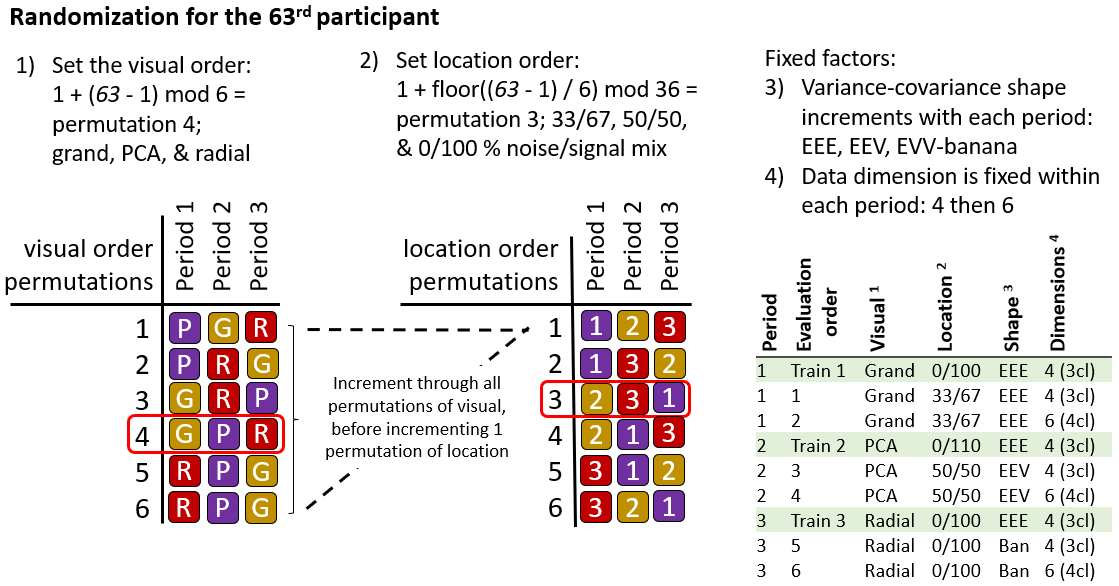
\includegraphics[width=1\linewidth]{./figures/figParmeterizationExample} 

}

\caption{Illustration of how a hypothetical participant 63 is assigned experimental factors. Each of the six visual order permutations is exhausted before iterating to the next permutation of location order.}\label{fig:figParmeterizationExample}
\end{figure}

\hypertarget{sec:demographics}{%
\subsection{Participant demographics}\label{sec:demographics}}

The target population is relatively well-educated people, as linear projections may prove difficult for generalized consumption. Hence, Prolific.co participants are restricted to those with an undergraduate degree (58,700 of the 150,400 users at the study time). From this cohort, 108 performed a complete study. Of these participants, 84 submitted the post-study survey, represented in the following heatmap. All participants were compensated for their time at \pounds 7.50 per hour, with a mean time of about 16 minutes. Figure \ref{fig:figSurveyDemographics} shows a heat map of the demographics for these 84 participants.

\begin{figure}

{\centering 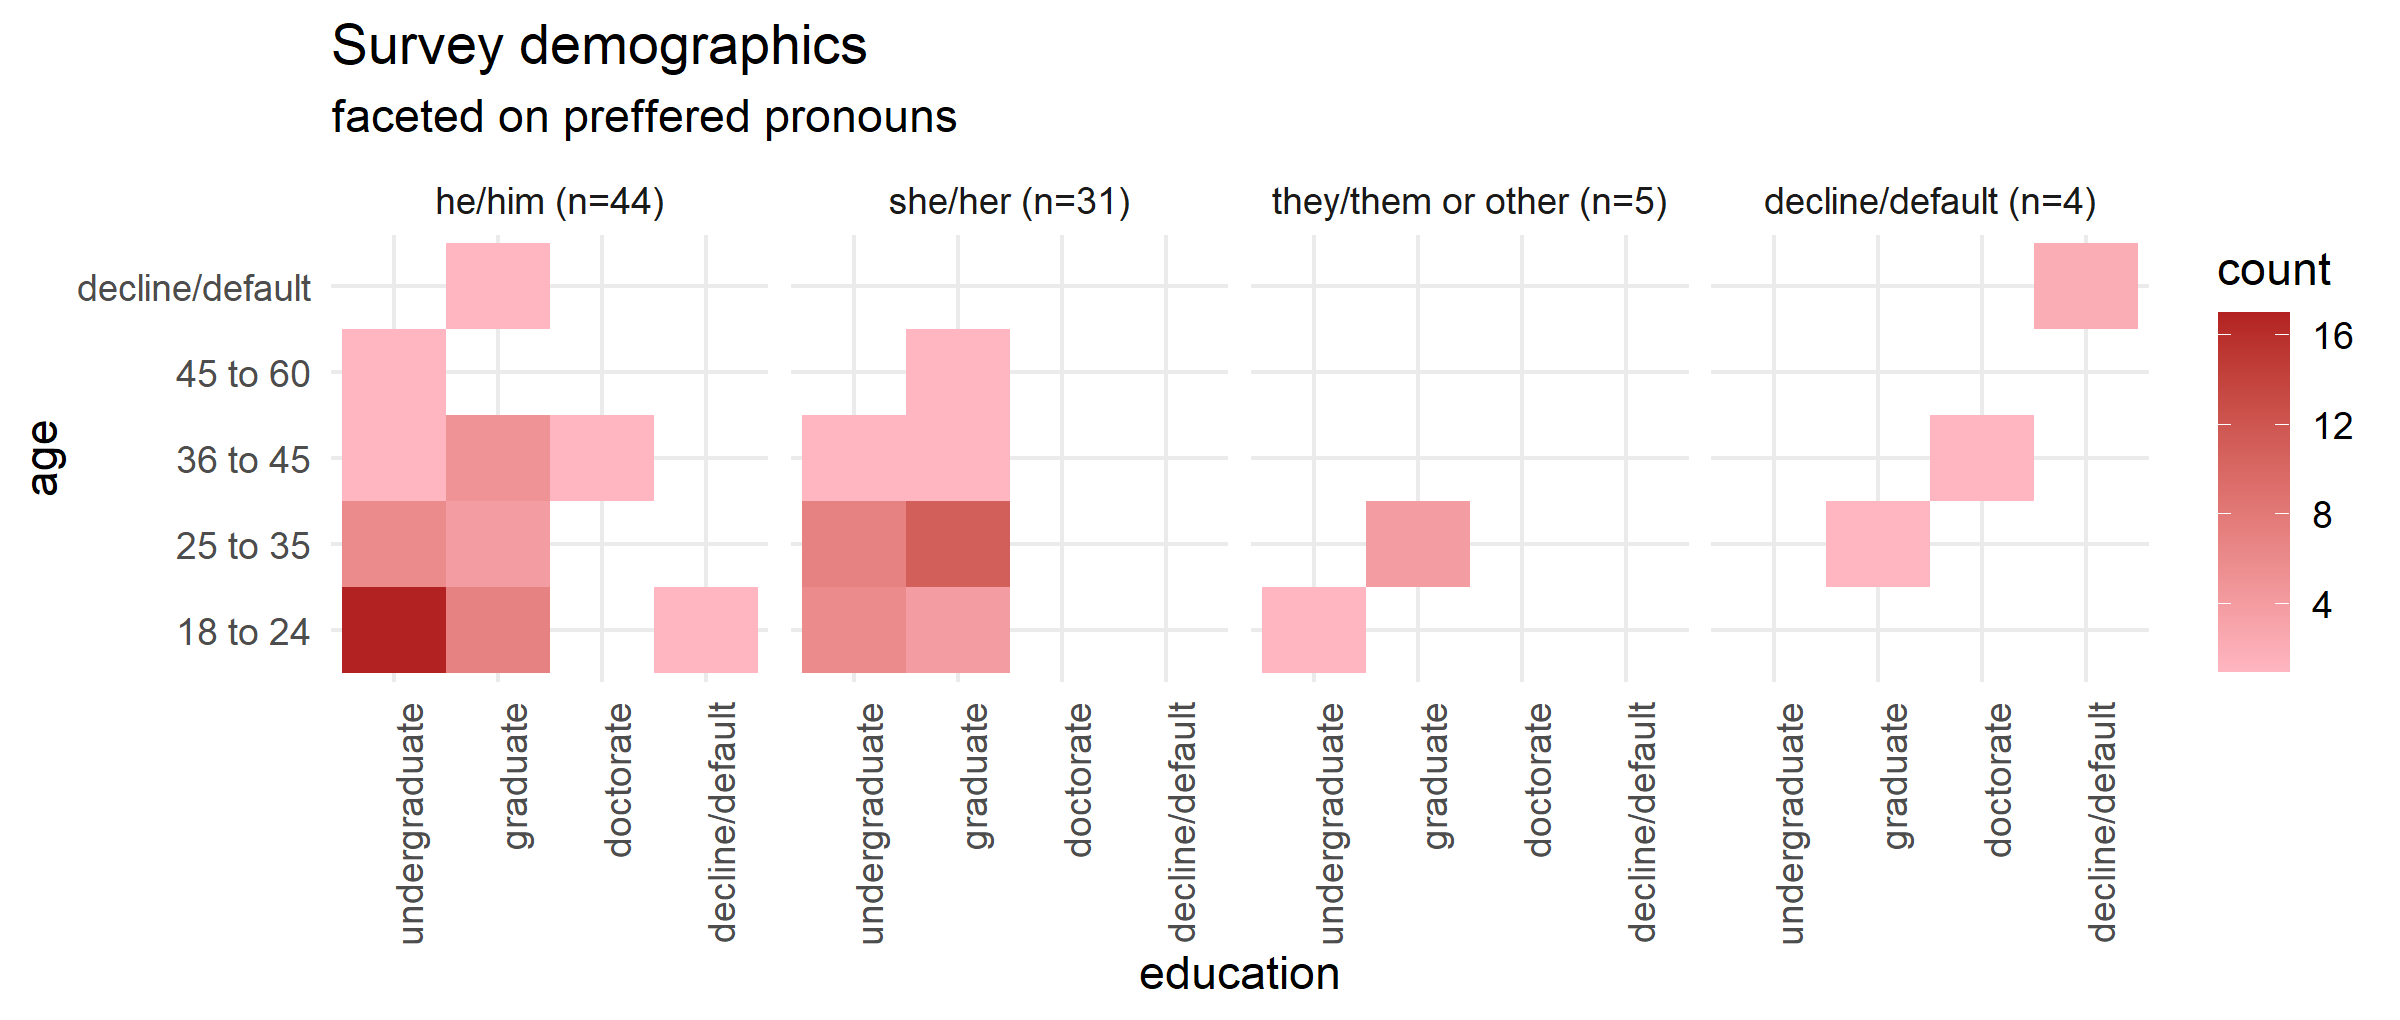
\includegraphics[width=1\linewidth]{./figures/figSurveyDemographics} 

}

\caption{Heatmaps of survey participant demographics; counts of age group by completed education as faceted across preferred pronouns. Our sample tended to be between 18 and 35 years of age with an undergraduate or graduate degree.}\label{fig:figSurveyDemographics}
\end{figure}

\hypertarget{sec:responsetime}{%
\subsection{Response time}\label{sec:responsetime}}

As a secondary explanatory variable, response time is considered. Response time is first log-transformed to remove its right skew. The same modeling procedure is repeated for this response. 1) Compare the performance of progressively more complex models. Table \ref{tab:timeCompTbl} shows the higher level performance of these models over increasing model complexity. 2) Select the model with the same effect terms, \(\alpha \times \beta + \gamma + \delta\), with relatively high conditional \(R^2\) without becoming overly complex from variable interactions. The coefficients of this model are displayed in Table \ref{tab:timeCoefTbl}.

\begin{table}

\caption{\label{tab:timeCompTbl}Model performance regressing on log response time [seconds], $\widehat{Y_2}$ random effect models. Conditional $R^2$ includes the random effects, while marginal does not. The model $\alpha \times \beta + \gamma + \delta$ model is selected to examine further as it has a relatively high marginal $R^2$ while having much less complexity than the complete interaction model.}
\centering
\fontsize{8}{10}\selectfont
\begin{tabular}[t]{lrrrrr}
\toprule
Model & AIC & BIC & R2 cond. & R2 marg. & RMSE\\
\midrule
\cellcolor{gray!6}{a} & \cellcolor{gray!6}{\textbf{1448}} & \cellcolor{gray!6}{\textbf{1448}} & \cellcolor{gray!6}{1474.771} & \cellcolor{gray!6}{0.645} & \cellcolor{gray!6}{0.643}\\
a+b+c+d & 1467 & 1467 & 1515.857 & 0.647 & \textbf{0.641}\\
\cellcolor{gray!6}{a*b+c+d} & \cellcolor{gray!6}{1474} & \cellcolor{gray!6}{1474} & \cellcolor{gray!6}{1540.803} & \cellcolor{gray!6}{0.656} & \cellcolor{gray!6}{0.647}\\
a*b*c+d & 1488 & 1491 & 1626.566 & 0.673 & 0.654\\
\cellcolor{gray!6}{a*b*c*d} & \cellcolor{gray!6}{1537} & \cellcolor{gray!6}{1548} & \cellcolor{gray!6}{\textbf{1791.707}} & \cellcolor{gray!6}{\textbf{0.7}} & \cellcolor{gray!6}{0.68}\\
\bottomrule
\end{tabular}
\end{table}

\begin{table}

\caption{\label{tab:timeCoefTbl}Model coefficients for log response time [seconds] $\widehat{Y_2} = \alpha \times \beta + \gamma + \delta$, with factor = pca, location = 0/100\%, shape = EEE, and dim = 4 held as baselines. Location = 50/50\% is the fixed term with the strongest evidence and takes less time. In contrast, the interaction term location = 50/50\%:shape = EEV has the most evidence and takes much longer on average.}
\centering
\fontsize{8}{10}\selectfont
\begin{tabular}[t]{lrrrrrl}
\toprule
  & Est & SE & df & t val & Prob & \\
\midrule
\cellcolor{gray!6}{(Intercept)} & \cellcolor{gray!6}{2.71} & \cellcolor{gray!6}{0.14} & \cellcolor{gray!6}{42.6} & \cellcolor{gray!6}{19.06} & \cellcolor{gray!6}{0.000} & \cellcolor{gray!6}{***}\\
\addlinespace[0.3em]
\multicolumn{7}{l}{\textbf{Factor}}\\
\hspace{1em}VisGrand & -0.23 & 0.12 & 567.6 & -1.97 & 0.049 & *\\
\cellcolor{gray!6}{\hspace{1em}VisRadial} & \cellcolor{gray!6}{0.16} & \cellcolor{gray!6}{0.12} & \cellcolor{gray!6}{573.5} & \cellcolor{gray!6}{1.34} & \cellcolor{gray!6}{0.181} & \cellcolor{gray!6}{}\\
\addlinespace[0.3em]
\multicolumn{7}{l}{\textbf{Fixed effects}}\\
\hspace{1em}Loc33/66\% & 0.05 & 0.14 & 40.9 & 0.34 & 0.737 & \\
\cellcolor{gray!6}{\hspace{1em}Loc50/50\%} & \cellcolor{gray!6}{-0.05} & \cellcolor{gray!6}{0.14} & \cellcolor{gray!6}{42.1} & \cellcolor{gray!6}{-0.35} & \cellcolor{gray!6}{0.729} & \cellcolor{gray!6}{}\\
\hspace{1em}ShapeEEV & -0.15 & 0.09 & 8.3 & -1.61 & 0.145 & \\
\cellcolor{gray!6}{\hspace{1em}ShapeBanana} & \cellcolor{gray!6}{-0.13} & \cellcolor{gray!6}{0.09} & \cellcolor{gray!6}{8.3} & \cellcolor{gray!6}{-1.42} & \cellcolor{gray!6}{0.192} & \cellcolor{gray!6}{}\\
\hspace{1em}Dim6 & 0.14 & 0.08 & 8.3 & 1.90 & 0.093 & \\
\addlinespace[0.3em]
\multicolumn{7}{l}{\textbf{Interactions}}\\
\cellcolor{gray!6}{\hspace{1em}VisGrand:Loc33/66} & \cellcolor{gray!6}{0.24} & \cellcolor{gray!6}{0.18} & \cellcolor{gray!6}{580.9} & \cellcolor{gray!6}{1.34} & \cellcolor{gray!6}{0.181} & \cellcolor{gray!6}{}\\
\hspace{1em}VisRadial:Loc33/66 & -0.24 & 0.18 & 582.4 & -1.32 & 0.188 & \\
\cellcolor{gray!6}{\hspace{1em}VisGrand:Loc50/50} & \cellcolor{gray!6}{0.12} & \cellcolor{gray!6}{0.18} & \cellcolor{gray!6}{578.6} & \cellcolor{gray!6}{0.69} & \cellcolor{gray!6}{0.491} & \cellcolor{gray!6}{}\\
\hspace{1em}VisRadial:Loc50/50 & 0.05 & 0.18 & 584.4 & 0.25 & 0.800 & \\
\bottomrule
\end{tabular}
\end{table}

\end{document}
